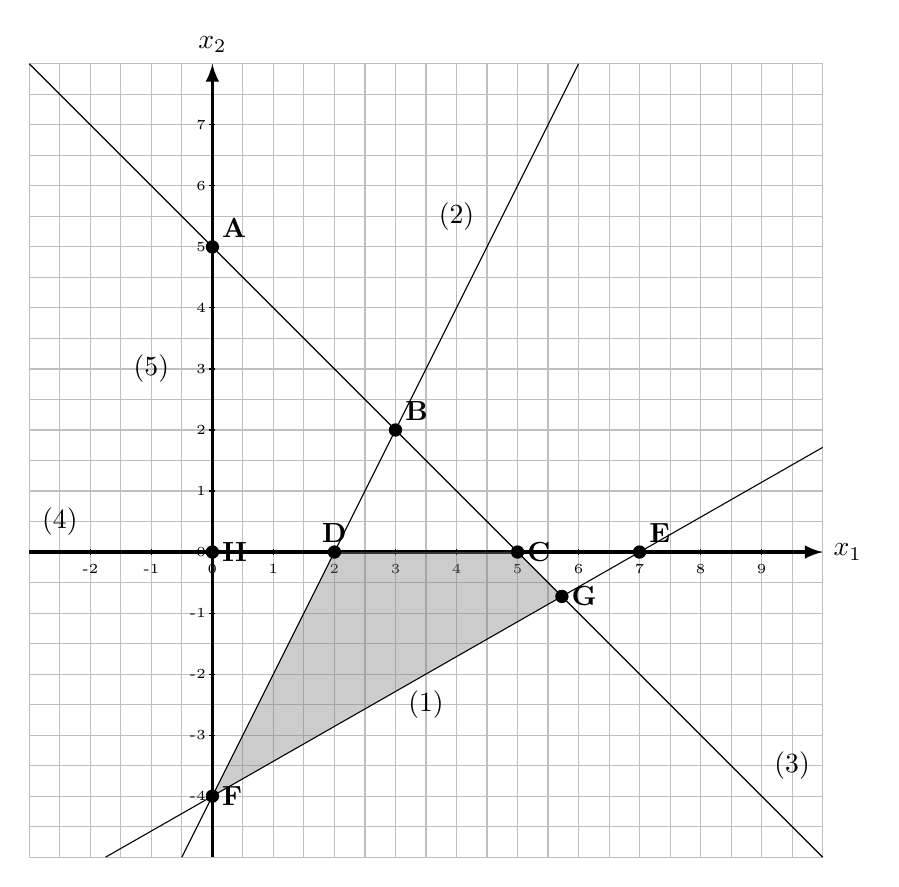
\begin{tikzpicture}[scale=0.775]
  \draw[gray!50, thin, step=0.5] (-3, -5) grid (10, 8);
  \draw[very thick, -latex] (-3, 0) coordinate(x1) -- (10, 0) coordinate(x2) node[right] {$x_1$};
  \draw[very thick, -latex] (0, -5) coordinate(y1) -- (0, 8) coordinate(y2) node[above] {$x_2$};
  \foreach \x in {-2, ..., 9} {
    \draw (\x, 0.05) -- (\x, -0.05) node[below] {\tiny\x};
    }
  \foreach \y in {-4, ..., 7} {
    \draw (-0.05, \y) -- (0.05, \y) node[left] {\tiny\y};
  }
  \fill[gray, opacity=0.4] (0, -4) -- (63/11, -8/11) -- (5, 0) -- (2, 0) -- cycle; 
  \draw (10, 12/7) -- (-7/4, -5);
  \draw (-1/2, -5) -- (6, 8);
  \draw (10, -5) -- (-3, 8);
  \node at (4, 5.5){(2)};
  \node at (3.5, -2.5){(1)};
  \node at (9.5, -3.5){(3)};
  \node at (-2.5, 0.5){(4)};
  \node at (-1, 3){(5)};
  
  \draw [draw=black, fill=black] (0, 5) circle (0.1) node[anchor=south west] {\textbf{A}};	
  \draw [draw=black, fill=black] (3, 2) circle (0.1) node[anchor=south west] {\textbf{B}};
  \draw [draw=black, fill=black] (5, 0) circle (0.1) node[anchor=west] {\textbf{C}};
  \draw [draw=black, fill=black] (2, 0) circle (0.1) node[anchor=south] {\textbf{D}};
  \draw [draw=black, fill=black] (7, 0) circle (0.1) node[anchor=south west] {\textbf{E}};
  \draw [draw=black, fill=black] (0, -4) circle (0.1) node[anchor=west] {\textbf{F}};
  \draw [draw=black, fill=black] (63/11, -8/11) circle (0.1) node[anchor=west] {\textbf{G}};
  \draw [draw=black, fill=black] (0, 0) circle (0.1) node[anchor=west] {\textbf{H}};
\end{tikzpicture}
